%% LyX 2.3.1-1 created this file.  For more info, see http://www.lyx.org/.
%% Do not edit unless you really know what you are doing.
\documentclass[english,hebrew]{article}
\usepackage[T1]{fontenc}
\usepackage[utf8]{inputenc}
\usepackage{babel}
\usepackage{amsmath}
\usepackage{amssymb}
\usepackage{graphicx}
\usepackage[unicode=true]
 {hyperref}

\makeatletter

%%%%%%%%%%%%%%%%%%%%%%%%%%%%%% LyX specific LaTeX commands.
\DeclareTextSymbolDefault{\textquotedbl}{T1}

\makeatother

\begin{document}
\title{תורת הקבוצות - הרכבת פונקציות ויחסים}
\maketitle
\begin{description}
\item [{קטגוריות:}] תורת הקבוצות
\item [{תגים:}] תורת הקבוצות, פונקציות
\item [{מזהה:}] \L{\textbf{function\_and\_relation\_composition}}
\end{description}
בסדת הפוסטים שלי על תורת הקבוצות הכרנו יחסים והכרנו פונקציות. זה נותן
לנו אבני לגו, וכידוע מה שעושים עם אבני לגו הוא לחבר אותן אחת לשניה.
בהקשר של פונקציות המשמעות של חיבור שכזה היא פשוטה: אנחנו רוצים להפעיל
פונקציה אחת על \textbf{הפלט} של הפונקציה השניה. כלומר, אם אני חושב
על פונקציה בתור מין קופסה שחורה שכזו שיש לה צינור כניסה של \textquotedblright קלט\textquotedblleft{}
וצינור יציאה של \textquotedblright פלט\textquotedblleft , אז המשמעות
של הרכבה של פונקציות היא לחבר את צינור הקלט של הפונקציה השניה לצינור
הפלט של הפונקציה הראשונה, ככה:

\textbf{\L{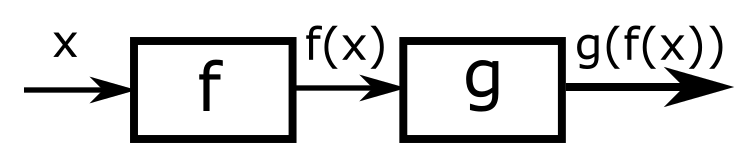
\includegraphics{C:/Users/gadia/Dropbox/Websites/blog/assets/img/2020/05/function_composition.PNG}}}

ברמת הסימון זה פשוט מאוד: אם \L{$f,g$} הן פונקציות, אני יכול לכתוב
\L{$g\left(f\left(x\right)\right)$} במשמעות של \textquotedblright מפעילים
את \L{$g$} על התוצאה של הפעלת \L{$f$} על \L{$x$}\textquotedblleft .
כדי לפשט את הסימון אפשר להשמיט את הסוגריים ופשוט לכתוב \L{$gf\left(x\right)$}
באותה משמעות בדיוק. לפעמים גם כותבים \L{$g\circ f\left(x\right)$}
במשמעות הזו, אבל אני לא אוהב את הסימון הזה ועוד נחזור לכך בהמשך. לסיום,
אפשר לכתוב פשוט \L{$gf$} כדי לתאר את הפונקציה שמתקבלת מההרכבה הזו
של \L{$g$} על \L{$f$}: כלומר הפונקציה שלכל \L{$x$} מחזירה את \L{$g\left(f\left(x\right)\right)$}.

עד כאן האינטואיציה, אבל מה עם הפורמליזם? צריך קצת להיזהר. לא כל שתי
פונקציות אפשר להרכיב. כדי שתהיה משמעות להרכבה כזו, \textbf{הפלט} של
\L{$f$} צריך להיות משהו שיהיה \textbf{קלט חוקי} עבור \L{$g$}. כזכור,
כל פונקציה באה עם שתי קבוצות כחלק מההגדרה שלה: קבוצה \L{$A$} שנקראת
\textbf{התחום} של הפונקציה )המקום שממנו נלקחים הקלטים( וקבוצה \L{$B$}
שנקראת \textbf{הטווח} של הפונקציה )זו קבוצה שכל הפלטים נמצאים בתוכה,
אבל ייתכן שיש בה עוד איברים שאינם מתקבלים בתור פלט(. כדי שתהיה משמעות
להרכבת הפונקציה \L{$g$} על \L{$f$} אנחנו רוצים שהתחום של \L{$g$}
יהיה שווה לטווח של \L{$f$}, כלומר שהפונקציות יהיו \L{$f:A\to B$}
ו-\L{$g:B\to C$}. במקרה הזה, הפונקציה שמתקבלת מההרכבה היא פונקציה
\L{$gf:A\to C$} - הקבוצה \L{$B$} ששימשה בתור מין \textquotedblright מתווך\textquotedblleft{}
בין \L{$f$} ו-\L{$g$} נעלמה לגמרי.

אפשר להקל קצת על הדרישה הזו שהתחום יהיה שווה לטווח: כל מה שאנחנו צריכים
מ-\L{$f$} הוא שכל \textbf{פלט שהיא מוציאה בפועל} יהיה שייך לתחום
של \L{$g$}. הטווח של \L{$f$} יכול להיות עצום וגדול וחורג בהרבה מהתחום
של \L{$g$} ועדיין לא תהיה בעיה להרכיב את שתיהן. התנאי המדויק, אם
כן, הוא שאם \L{$g:B\to C$} ו-\L{$A$} הוא התחום של \L{$f$}, אז מתקיים
\L{$f\left(A\right)\subseteq B$} )\textquotedblleft\textbf{התמונה}
של \L{$f$} מוכלת בתחום של \L{$g$}\textquotedblleft (.

בואו נראה כמה דוגמאות פשוטות. למשל, \L{$f,g:\mathbb{R}\to\mathbb{R}$}
שמוגדרות על ידי \L{$f\left(x\right)=x^{2}$} ו-\L{$g\left(x\right)=x+3$}.
קל לראות ש-\L{$gf\left(x\right)=x^{2}+3$} ו-\L{$fg\left(x\right)=\left(x+3\right)^{2}=x^{2}+6x+9$},
וזה גם מראה לנו שהרכבת פונקציות \textbf{היא לא קומוטטיבית}: כלומר,
\L{$fg$} ו-\L{$gf$} יהיו בדרך כלל פונקציות שונות )ושימו לב שלא בהכרח
שתיהן קיימות בכלל - זה תלוי בתחומים והטווחים של הפונקציות(.

הנה דוגמא קצת יותר מטורללת: ניקח בתור \L{$f$} את הפונקציה שעושה איחוד
של קבוצות - כלומר, הקלט שלה יהיה זוג של קבוצות והפלט שלה יהיה קבוצה
בודדת. פורמלית, אם \L{$U$} הוא \textquotedblright העולם\textquotedblleft{}
שלנו שכל הקבוצות הרלוונטיות הן תת-קבוצות שלו, אז \L{$f:2^{U}\times2^{U}\to2^{U}$}
זו הדרך שלי לכתוב ש-\L{$f$} לוקחת זוג )זה ה-\L{$\times$}( של תת-קבוצות
של \L{$U$} )זה ה-\L{$2^{U}$}( ומחזירה תת-קבוצה של \L{$U$}, ו-\L{$f$}
מוגדרת על ידי \L{$f\left(A,B\right)=A\cup B$}. עכשיו, ניקח בתור \L{$g$}
את הפונקציה שמקבלת קבוצה בודדת )לא זוג!( ומחזירה את קבוצת החזקה שלה,
כלומר \L{$g\left(A\right)=2^{A}$}. אז \L{$gf\left(A,B\right)=2^{A\cup B}$}
ואילו \L{$fg$} בכלל לא מוגדרת.

עכשיו בואו נחזור שניה לפוסט הקודם. ראינו שם שאם \L{$f:A\to B$} היא
פונקציה חד-חד-ערכית ועל, אז קיימת פונקציה \L{$f^{-1}:B\to A$} בעלת
התכונה הבאה: \L{$f\left(x\right)=y$} אם ורק אם \L{$f^{-1}\left(y\right)=x$}.
קל לראות שההרכבה מקיימת \L{$f^{-1}f\left(x\right)=x$}, וזו הזדמנות
להציג טרמינולוגיה חדשה.

אם \L{$A$} היא קבוצה כלשהי, אז \textbf{פונקציית הזהות} על \L{$A$}
היא הפונקציה \L{$I_{A}:A\to A$} שמקיימת \L{$I_{A}\left(x\right)=x$}
לכל \L{$x\in A$}. מה שראינו לפני רגע הוא ש-\L{$f^{-1}f=I_{A}$}.
יש הרבה דמיון בין המשוואה הזו ובין כפל \textquotedblright רגיל\textquotedblleft :
אם אנחנו חושבים על \L{$I_{A}$} בתור המספר {\beginL 1\endL} )למה {\beginL 1\endL}?
כי {\beginL 1\endL} הוא המספר שכפל בו לא משנה את האיבר שהוכפל, בדומה
לאיך שפונקצית הזהות לא משנה את הקלט שלה(, על \L{$f$} בתור מספר כלשהו
\L{$a$} ועל \L{$f^{-1}$} בתור \L{$\frac{1}{a}$} ועל הרכבת פונקציות
בתור כפל \textquotedblright רגיל\textquotedblleft , אז השוויון \L{$f^{-1}f=I_{A}$}
מזכיר לנו את השוויון \L{$\frac{1}{a}\cdot a=1$}. הדמיון הזה מסביר
את שיטת הסימון שבה בחרנו לתאר את \L{$f^{-1}$} וגם לתת אינטואיציה
למובן שבו היא \textquotedblright הופכית\textquotedblleft .

עכשיו, שימו לב למשהו טריקי קצת. מהי \L{$ff^{-1}$}? גם זו פונקצית
הזהות, אבל \textbf{איזו} פונקציית זהות? אם תחשבו על זה רגע תראו ש-\L{$ff^{-1}=I_{B}$}
. זו פונקציית הזהות \textbf{על קבוצה אחרת}, כי הפכנו את הסדר בין הקלטים
לפלטים )\L{$ff^{-1}$} היא פונקציה שבה \L{$f^{-1}$} פועלת ראשונה,
ולכן הקלט הוא מתוך \L{$B$}(.

בואו נראה דוגמא קונקרטית לזה - כאן תבוא לעזרתנו הפונקציה \L{$\text{tan}$},
טנגנס. לא חייבים לדעת בדיוק איך מוגדרת טנגנס; מספיק טוב לדעת שזו פונקציה
שהתחום שלה הוא \L{$\left(-\frac{\pi}{2},\frac{\pi}{2}\right)$} והטווח
שלה הוא \L{$\mathbb{R}$} והיא חח\textquotedblleft ע ועל, ולכן קיימת
לה הופכית \L{$\tan^{-1}$} שמכונה גם \textquotedblright ארקטנגנס\textquotedblleft ,
\L{$\text{arctan}$}. כעת, \L{$\text{arctan}\left(\text{tan}\right)$}
היא פונקציה עם תחום וטווח \L{$\left(-\frac{\pi}{2},\frac{\pi}{2}\right)$}
בזמן ש-\L{$\text{tan}\left(\text{arctan}\right)$} היא בעלת תחום וטווח
\L{$\mathbb{R}$}.

עכשיו בואו נשכח לרגע מפונקציות ונעבור לדבר על יחסים באופן כללי - אפשר
לדבר על \textquotedbl הרכבה\textquotedbl{} גם בהקשר הזה. נתחיל מהאינטואיציה:
הארי פוטר. בספרי הארי פוטר, הארי הוא הבן של לילי פוטר; ולילי פוטר
היא אחותה של פטוניה דרסלי. זה אומר שפטוניה היא דודתו של הארי. כל זה
איכשהו גם רלוונטי לעלילה אבל בואו נסתכל על זה מנקודת מבט מתמטית. יש
לנו שני יחסים שמוגדרים על קבוצת בני האדם: היחס \textquotedblright להיות
אחות של\textquotedblleft{} והיחס \textquotedbl להיות הורה של\textquotedblleft .
בואו נסמן את \textquotedblright להיות אחת של\textquotedblleft{} ב-\L{$R$}
ואת \textquotedblright להיות הורה של\textquotedblleft{} ב-\L{$S$},
ועכשיו נסמן את פטוניה ב-\L{$a$}, את לילי ב-\L{$b$} ואת הארי ב-\L{$c$},
ואנחנו רואים ש\textquotedblleft פטוניה היא אחותה של לילי\textquotedblleft{}
מתורגם ל-\L{$\left(a,b\right)\in R$} ו\textquotedblleft לילי היא
הורה של הארי\textquotedblleft{} מתורגם ל-\L{$\left(b,c\right)\in S$}.

עכשיו משני אלו אנחנו מסיקים שפטוניה היא הדודה של הארי, מה שאני יכול
לסמן ב-\L{$\left(a,c\right)\in T$} כאשר \L{$T$} הוא היחס \textquotedblright להיות
דודה של\textquotedblleft . מה הקשר בין היחסים \L{$R,S$} ובין היחס
\L{$T$}? אני רוצה לומר שהוא קשר של \textbf{הרכבה}; הרי ההגדרה של
\textquotedblright להיות דודה של\textquotedblleft{} היא בדיוק \textquotedblright להיות
אחות של הורה של\textquotedblleft . אז בואו ננסה לתת הגדרה להרכבת יחסים
שתשמר את האינטואיציה הזו.

נניח שנתונים לנו שני יחסים, \L{$R,S$}, כך ש-\L{$R\subseteq A\times B$}
ו-\L{$S\subseteq B\times C$}. אפשר לתאר אותם גרפית בצורה הזו:

\textbf{\L{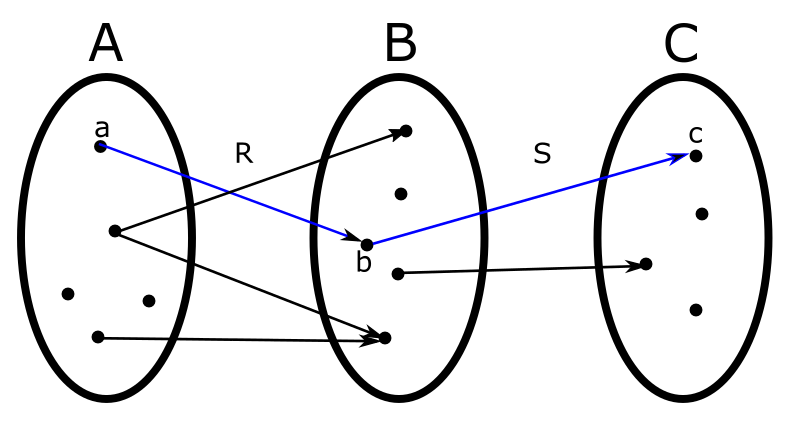
\includegraphics{C:/Users/gadia/Dropbox/Websites/blog/assets/img/2020/05/relation_composition.PNG}}}

באיור הזה הקבוצות \L{$A,B,C$} מיוצגות כולן על ידי אליפסות עם נקודות
בתוכן - כל נקודה מייצגת איבר של הקבוצה. את העובדה ש-\L{$\left(a,b\right)\in R$}
אני מייצג על ידי חץ שיוצא מ-\L{$a$} ונכנס אל \L{$b$} )ובדומה בתמונה
גם עשיתי חץ מ-\L{$b\in B$} אל \L{$c\in C$} כדי להמחיש ש-\L{$\left(b,c\right)\in S$}(.
חשוב היה לי להדגיש שהיחסים \L{$R,S$} הללו הם לא בהכרח פונקציות, אז
כללתי באיור נקודות ש\textquotedblleft מקלקלות\textquotedblleft{} את
התכונות של פונקציות: יש נקודה שממנה יוצאים שני חצים )מקלקל את ה\textquotedblleft יחידות\textquotedblleft (
ונקודה שממנה לא יוצאים חצים בכלל )מקלקל את ה\textquotedblleft קיום\textquotedblleft (.

עכשיו, סימנתי בכחול את החצים שמחברים את \L{$a$} אל \L{$b$} ואת \L{$b$}
אל \L{$c$} כי שילוב שני החצים הללו יוצר משהו מעניין - הוא יוצר \textbf{מסלול}
שמוביל אותנו מ-\L{$a$} אל \L{$c$} תוך מעבר ב\textquotedblleft איבר
הביניים\textquotedblleft{} \L{$b$}. זה בדיוק מה שהרכבת יחסים מנסה
לתפוס - מצבים כאלו שבהם קיים מסלול מנקודה אחת אל השניה בעזרת נקודת
ביניים\textbf{ כלשהי}. שימו לב שלא מעניין אותי אם יש יותר מנקודת ביניים
אפשרית אחת - אם פטוניה הייתה גם אחותו של ג'יימס פוטר בנוסף לכך שהיא
אחותה של לילי פוטר, היא עדיין הייתה דודה של הארי )אבל הספר עצמו היה
מקבל טוויסט מוזר למדי(. לכן ההגדרה להרכבת פונקציות תתבסס על הכמת הלוגי
\textquotedblright קיים\textquotedblleft{} )שאני מסמן ב-\L{$\exists$}(.

אחרי כל ההקדמה הזו הנה סוף סוף ההגדרה:

\L{$R\circ S\triangleq\left\{ \left(a,c\right)\ |\ \exists b\in B:\left(a,b\right)\in R\wedge\left(b,c\right)\in S\right\} $}

ובמילים: היחס המורכב \L{$R\circ S$} כולל את כל הזוגות \L{$\left(a,c\right)$}
כך שקיים איבר ביניים \L{$b\in B$} שעבורו \L{$\left(a,b\right)\in R$}
)\textquotedblleft הצעד הראשון\textquotedblleft ( ו-\L{$\left(b,c\right)\in S$}
)\textquotedblleft הצעד השני\textquotedblleft (. מצד אחד, זו הגדרה
פשוטה, כשמבינים מה היא מנסה להשיג; ומצד שני לטעמי זו אחת ההגדרות הקשות
ביותר בשלב הזה של לימודי תורת הקבוצות.

עכשיו אני צריך בלב כואב לדבר על שיטת הסימון שבחרתי להשתמש בה. אם תסתכלו
באיור, אפשר לראות ש-\L{$R$} היא בצד שמאל ו-\L{$S$} בצד ימין. זה
בכוונה; זה תואם את האופן שבו בתוך זוג סדור כמו \L{$\left(a,b\right)$}
ה\textquotedblleft כיוון\textquotedblleft{} הוא מ-\L{$a$} אל \L{$b$}.
זה הוביל אותי לסמן את ההרכבה, \L{$R\circ S$}, בצורה כזו שהאיבר שפועל
\textbf{קודם} )\L{$R$}, שמעביר איבר של \L{$A$} לאיבר של \L{$B$}(
נמצא בצד שמאל. זה \textbf{הפוך לגמרי} לסימון שבו השתמשתי \textbf{לפני
רגע בפוסט הזה} כשדיברתי על הרכבת פונקציות. שם, \L{$gf$} משמעותו הייתה
\textquotedblright קודם להפעיל את \L{$f$} ואז את \L{$g$}\textquotedblleft{}
כי ככה זה עובד עם סימון הפעלת פונקציות: \L{$g\left(f\left(x\right)\right)$}
אומר בדיוק שקודם מפעילים את \L{$f$} ואז את \L{$g$}.

העניין הוא שפונקציות \textbf{הן יחסים} והרכבת פונקציות \textbf{היא
הרכבת יחסים}. אז יש לי שני סימונים שונים \textbf{והפוכים} לאותו דבר.
ומילא אם זה היה רק אצלי, אבל כל טקסט מתמטי שמתעסק גם בהרכבת פונקציות
וגם בהרכבת יחסים ייאלץ להתמודד עם הניג'וס הזה.

פתרון נפוץ מאוד הוא פשוט להגדיר הרכבת יחסים הפוך, כמו הרכבת פונקציות:
\L{$S\circ R$} יתאר את מה שכתבתי עד כה למעלה. פתרון אחר, שבו אני
נוקט, הוא פשוט לא לסמן הרכבת פונקציות עם \L{$\circ$} ולשמור את הסימן
הזה להרכבת יחסים )כלומר, \L{$f\circ g$} יהיה התיאור שלי להרכבת הפונקציות
\L{$f,g$} כשאני חושב עליה בתור הרכבת יחסים; זה אומר ש-\L{$f\circ g\equiv gf$}(.
כמו רוב ענייני הסימון במתמטיקה זה לא \textbf{באמת} חשוב מה בוחרים,
כל עוד זה מוסבר מספיק ברור כדי לא להטעות את הקוראים.

אחרי שסילקנו את זה מהדרך, בואו נעשה קצת כיף! 

התכונה החשובה ביותר של הרכבת יחסים ופונקציות, שאחראית לתכונות האלגבריות
שלה שנראה בהמשך, היא \textbf{אסוציאטיביות}. כלומר, אם יש לנו הרכבה
של \textbf{שלושה} יחסים שמתוארת בתור זוג הרכבות, \L{$R\circ S\circ T$},
זה לא משנה איזו מההרכבות אנחנו מבצעים קודם - תמיד נקבל בסוף את אותו
יחס. פורמלית, \L{$\left(R\circ S\right)\circ T=R\circ\left(S\circ T\right)$}.
ההוכחה של זה מייגעת למדי וכמובן שאדלג עליה )\textquotedblleft להשאיר
את הוכחת האסוציאטיביות כתרגיל לקורא\textquotedblleft{} זו שיטת הפעולה
של כל טקסט מתמטי מיום שהומצאה האלגברה( אבל האינטואיציה פה די פשוטה
כשחוזרים לחשיבה על הרכבת יחסים בתור \textquotedblright למצוא נקודות
שמחבר ביניהן מסלול\textquotedblleft{} כי קיום מסלול לא תלוי בשאלה אם
קודם אנחנו מסתכלים על שלוש הנקודות הראשונות שבו )\L{$R\circ S$}(
או שלוש הנקודות האחרונות )\L{$S\circ T$}(.

עכשיו, מרגע שהמתמטיקאים ממציאים פעולה, הם רוצים לבצע אותה שוב ושוב
כמה שרק אפשרי. במקרה הזה אפשר לדבר על זה כאשר מרכיבים יחס \textbf{עם
עצמו}. כדי שאפשר יהיה לעשות את זה, צריך שהתחום והטווח של היחס יהיו
אותה קבוצה. כלומר, ניקח יחס \L{$R\subseteq A\times A$} וכעת אפשר
להגדיר \L{$R^{2}=R\circ R$} ו-\L{$R^{3}=R\circ R\circ R$} וכדומה.
בואו ניתן הגדרה אפילו יותר פורמלית.

ראשית, אני משתמש בסימון של חזקה לא במקרה; זה המשך של האנלוגיה בין
הרכבה ובין כפל. אז בואו ניזכר איך מגדירים חזקה טבעית במספרים ממשיים:
ראשית מגדירים \L{$a^{0}\triangleq1$} לכל \L{$a$} )כן, \L{\href{https://gadial.net/2018/01/01/zero_power_equals_one/}{אני מגדיר ככה}}
אפילו עבור \L{$a=0$}(. כעת מגדירים אינדוקטיבית \L{$a^{n+1}\triangleq a\cdot a^{n}$}.
המשמעות של לומר \textquotedblright מגדירים אינדוקטיבית\textquotedblleft{}
היא שמניחים ש-\L{$a^{n}$} כבר הוגדר, ועכשיו משתמשים בו כדי להגדיר
את \L{$a^{n+1}$}. למשל אם כבר הגדרתי את \L{$a^{3}$} אז \L{$a^{4}$}
יוגדר להיות \L{$a^{3}\cdot a$}.

ההגדרה של חזקה של יחס תהיה זהה, אבל אנחנו צריכים אנלוג ל-\L{$1$}.
כבר היה לנו כזה במקרה של פונקציות - פונקציית הזהות. אז בואו ניקח את
הפונקציה הזו ונחשוב עליה בתור יחס:

\L{$I_{A}\triangleq\left\{ \left(a,a\right)|\ a\in A\right\} $}

ועכשיו אפשר לתת פורמלית את ההגדרה האינדוקטיבית:

\L{$R^{0}\triangleq I_{A}$}

\L{$R^{n+1}\triangleq R\circ R^{n}$}

קל לראות ש-\L{$R^{1}=R$} בהגדרה הזו, בצורה עקבית עם מה שאנחנו רגילים
שחזקת {\beginL 1\endL} עושה. יותר מזה, אפשר לראות גם שחוקי החזקות
הרגילים מתקיימים: \L{$R^{n+m}=R^{n}\circ R^{m}$} ו-\L{$R^{nm}=\left(R^{n}\right)^{m}$}.
ההוכחה קצת מייגעת אבל לא באמת שונה מההוכחה עבור חוקי החזקות הרגילים
- מילת המפתח שגורמת לדברים להתנהג דומה היא ה\textbf{אסוציאטיביות}
של פעולת ההרכבה.

זה היה נחמד, אבל צריך להיזהר לא לקחת את ההקבלה יותר מדי רחוק - כשמגיעים
לחזקות \textbf{שליליות} דברים מוזרים מתחילים לקרות. ראשית, איך אני
מגדיר חזקה שלילית? כבר ראינו את ההגדרה \L{$R^{-1}\triangleq\left\{ \left(b,a\right)\ |\ \left(a,b\right)\in R\right\} $}.
עכשיו אפשר להשתמש בה כדי להגדיר חזקה שלילית כללית: \L{$R^{-n}\triangleq\left(R^{-1}\right)^{n}$}.
כלומר, לוקחים את היחס \L{$R^{-1}$} )שהוא יחס טוב ונחמד שקיים בזכות
עצמו( ואז מסתכלים על החזקה ה-\L{$n$}-ית שלו.

כל זה סבבה, אבל שימו לב שממש לא בהכרח מתקיים \L{$R\circ R^{-1}=I_{A}$},
כלומר \L{$R^{-1}$} הוא לא הופכי של \L{$R$} במובן האלגברי של המילה.
למשל, אם \L{$A=\left\{ 1,2\right\} $} ו-\L{$R=\left\{ \left(1,2\right)\right\} $}
אז \L{$R\circ R^{-1}=\left\{ \left(1,1\right)\right\} $} וזה בוודאי
לא \L{$I_{A}$} כי \L{$\left(2,2\right)\in I_{A}$}, כלומר עשויים
להיות חסרים לי איברים. גרוע מכך, עשויים לצוץ לי איברים שלא אמורים
להיות שם: למשל אם \L{$A=\left\{ 1,2,3\right\} $} ו-\L{$R=\left\{ \left(2,1\right),\left(3,1\right)\right\} $}
אני אקבל \L{$\left(2,3\right)\in R\circ R^{-1}$}. זה כמובן מצער מאוד,
אבל תראו, קסם! אם \L{$R$} היא \textbf{פונקציה הפיכה} אז לא קשה להוכיח
שכן יתקיים \L{$R\circ R^{-1}=I_{A}$} וזה מוביל לכך שלפונקציות הפיכות
יש מבנה אלגברי מאוד יפה שבו מעורבת פעולה אסוציאטיבית עם איבר אדיש
והופכי - מה שנקרא \textbf{חבורה}. אבל זה סיפור אחר \L{\href{https://gadial.net/2017/02/01/group_definition/}{ויסופר בפעם אחרת}}.

עכשיו, אחרי שטיפה התרגלנו לחזקות של יחסים, בואו נחזור אל התכונות הנחמדות
שהגדירו יחס שקילות - רפלקסיביות, סימטריה וטרנזיטיביות. כל אחת מהן
ניתנת לניסוח פשוט באמצעות חזקות של יחסים:
\begin{enumerate}
\item רפלקסיביות של \L{$R\subseteq A\times A$} פירושה ש-\L{$\left(a,a\right)\in R$}
לכל \L{$a\in A$}. כלומר, זה פשוט אומר ש-\L{$I_{A}\subseteq R$},
או במילים אחרות \L{$R^{0}\subseteq R$}.
\item סימטריה של \L{$R\subseteq A\times A$} פירושה שאם \L{$\left(a,b\right)\in R$}
אז גם \L{$\left(b,a\right)\in R$}. כלומר, ש-\L{$R^{-1}\subseteq R$}.
\item טרנזיטיביות של \L{$R\subseteq A\times A$} פירושה שאם \L{$\left(a,b\right)\in R$}
וגם \L{$\left(b,c\right)\in R$} אז גם \L{$\left(a,c\right)\in R$}.
כלומר, זה פשוט אומר ש-\L{$R^{2}\subseteq R$} )ומכך נובע \L{$R^{n}\subseteq R$}
לכל \L{$n\ge2$}(.
\end{enumerate}
אם כל התכונות הללו מתקיימות גם יחס אז \L{$R$} הוא יחס שקילות, והנה
קיבלנו דרך אחרת לתאר יחס שקילות, באמצעות חזקות: \L{$R$} הוא יחס שקילות
אם ורק אם \L{$R^{k}\subseteq R$} לכל \L{$k\in\mathbb{Z}$}.

לסיום, אני לא יכול להתאפק וחייב להכניס פנימה עוד קשר מתמטי שעשוי להישמע
מוזר ממבט ראשון אבל כשחושבים עליו רגע הוא מובן מאליו לגמרי - הרכבת
יחסים ממש מזכירה כפל מטריצות. אם אתם לא מכירים או זוכרים כפל מטריצות,
יש לי \L{\href{https://gadial.net/2011/10/06/matrix_product/}{פוסט על זה}}
כאן, ועכשיו אניח שכן מכירים את הרעיון, אבל אזכיר את ההגדרה: בכפל מטריצות
יש לנו שתי מטריצות \L{$R,S$} מעל חוג מסויים )כלומר, משהו שמוגדרות
עליו פעולות חיבור וכפל(. כדי לכפול אותן, צריך ש-\L{$R$} תהיה ממימד
\L{$n\times m$} ו-\L{$S$} ממימד \L{$m\times t$} )כלומר, מספר העמודות
של \L{$R$} יהיה שווה למספר השורות של \L{$S$}( ואז מגדירים \L{$\left[RS\right]_{ij}=\sum_{k=1}^{m}\left[R\right]_{ik}\left[S\right]_{kj}$}.
אני אפילו אכתוב את זה קצת יותר במפורש כך שרואים את פעולות החיבור והכפל:

\L{$\left[RS\right]_{ij}=\left[R\right]_{i1}\cdot\left[S\right]_{1j}+\cdots+\left[R\right]_{1m}\left[S\right]_{mj}$}

איך זה קשור ליחסים? ובכן, נניח שיש לי יחסים \L{$R\subseteq A\times B$}
ו-\L{$S\subseteq B\times C$}, כך ש-\L{$A,B,C$} כולן קבוצות סופיות.
נסמן את האיברים שלהן: \L{$A=\left\{ a_{1},\dots,a_{n}\right\} $}
ו-\L{$B=\left\{ b_{1},\dots,b_{m}\right\} $} ו-\L{$C=\left\{ c_{1},\dots,c_{t}\right\} $}.
עכשיו אפשר לייצג יחס באמצעות מטריצה:

\L{$\left[R\right]_{ij}=\begin{cases}
1 & \left(a_{i},b_{j}\right)\in R\\
0 & \left(a_{i},b_{j}\right)\notin R
\end{cases}$}

\L{$\left[S\right]_{ij}=\begin{cases}
1 & \left(b_{i},c_{j}\right)\in S\\
0 & \left(b_{i},c_{j}\right)\notin S
\end{cases}$}

כלומר, המטריצות הללו חיות מעל החוג \L{$\mathbb{Z}_{2}$}. בחוג הזה
יש לנו את פעולות הכפל והחיבור הרגילות מודולו {\beginL 2\endL}, אבל
הן \textbf{לא יעניינו} אותנו הפעם אלא מה שאפשר לקבל מהן. בגלל שבחוג
הזה מתקיים ש-\L{$a^{2}=a$} לכל \L{$a$}, קוראים לו \textbf{חוג בוליאני}
ואפשר לקבל ממנו משהו שנקרא \textbf{אלגברה בוליאנית}. לא אכנס לפרטים
המלאים, אבל הרעיון הוא שאפשר להגדיר פעולות חדשות, \L{$a\wedge b=a\cdot b$}
ו-\L{$a\vee b=a+b+a\cdot b$} שמתנהגות מאוד נחמד - בהקשר של \L{$\mathbb{Z}_{2}$}
הפעולות הללו מתנהגות כמו \textquotedblright וגם\textquotedblleft{}
)עבור \L{$\wedge$}( ו\textquotedblleft או\textquotedblleft{} )עבור
\L{$\vee$}( שאנחנו מכירים מלוגיקה. צריך לשים לב שעם שתי הפעולות הללו
\L{$\mathbb{Z}_{2}$} \textbf{אינו} חוג, כי אין נגדי חיבורי לפעולת
ה-\L{$\vee$} )ולכן היא לא יכולה לתפקד בתור פעולת החיבור של חוג( לכן
אמרתי שנקבל דמיון לכפל מטריצות ולא ממש מקרה פרטי.

עכשיו, זוכרים את ההגדרה של הרכבת יחסים?

\L{$R\circ S\triangleq\left\{ \left(a,c\right)\ |\ \exists b\in B:\left(a,b\right)\in R\wedge\left(b,c\right)\in S\right\} $}

במקום לכתוב \L{$\exists$}, אפשר, במקרה שבו הקבוצות \L{$A,B,C$} סופיות,
לכתוב משהו יותר מפורש בשביל התנאי שבפנים:

\L{$\left[\left(a,b_{1}\right)\in R\wedge\left(b_{1},c\right)\in S\right]\vee\dots\vee\left[\left(a,b_{m}\right)\in R\wedge\left(b_{m},c\right)\in S\right]$}

ובמילים - או שאפשר לעבור מ-\L{$a$} אל \L{$c$} עם איבר הביניים \L{$b_{1}$},
או שאפשר לעבור עם \L{$b_{2}$} וכן הלאה, עד \L{$b_{m}$}.

כלומר, קיבלנו ש-\L{$\left[R\circ S\right]_{ij}$} מוגדר בדיוק כמו
כפל מטריצות, פרט לכך שאנחנו מחליפים את התפקידים של חיבור וכפל ב-\L{$\wedge$}
וב-\L{$\vee$}. חמוד? אני מקווה, וגם נותן אינטואיציות מסויימות, אבל
אני בעיקר מקווה שחמוד.
\end{document}
